\begingroup
\renewcommand\thechapter{A}
\titleformat{\chapter}[display]
{\normalfont\huge\bfseries}{}{20pt}{\Huge}
\setcounter{section}{0} 
\setcounter{figure}{0}

\chapter*{Appendix A - Model Training}
\addcontentsline{toc}{chapter}{Appendix A - Model Training}
\markboth{Appendix A}{}

Training convolutional neural networks is a highly intensive task, requiring substantial amounts of processing power,
meaning many have to turn to cloud service providers to train their models.
Many such options exist to find the necessary processing power to train an advanced CNN, such as Google Colab, which offers 
free (rate-limited) access to Tesla T4 GPUs. Personal experimentation has revealed that it can be difficult to leverage Colab 
when performing data augmentation, often encountering rate limitations resulting in forced session termination. Additionally,
model training can take a long time on these GPUs, and there is always the possibility of a sudden internet connection loss that could 
cause all work to be lost.

\para Therefore, which Colab likely could be suitable for training the proposed model, it is instead also 
possible to leverage a local GPU which will be able to train the model at a substantially faster rate.
The proposed training method will be a local Jupyter Notebook running on a desktop PC with an AMD Radeon RX 9070 XT graphics card.
This GPU is not only substantially faster than a Tesla T4 as per \textcite{hardwaredbTeslaT4Vs,technicalcityRX9070XT} as well as personal 
anecdotal experimentation seen in Figures \ref{fig:GPUComparisonA} and \ref{fig:GPUComparisonB},
but would also not impose rate limits due to it being personally owned. This should allow for the model to be trained much faster, while not 
having to depend on cloud service availability.

\begin{figure}[H]
    \centering
    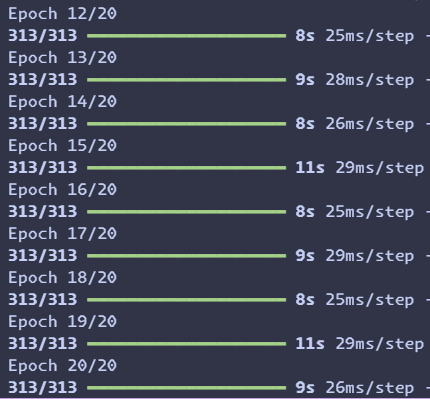
\includegraphics[width=0.5\textwidth]{Proposal/ColabModelTraining.png}
    \caption{Training time for a CNN on the CIFAR10 dataset using Colab (Approx. 27ms/step, 8-11s/epoch).\label{fig:GPUComparisonA}}
\end{figure}

\begin{figure}[H]
    \centering
    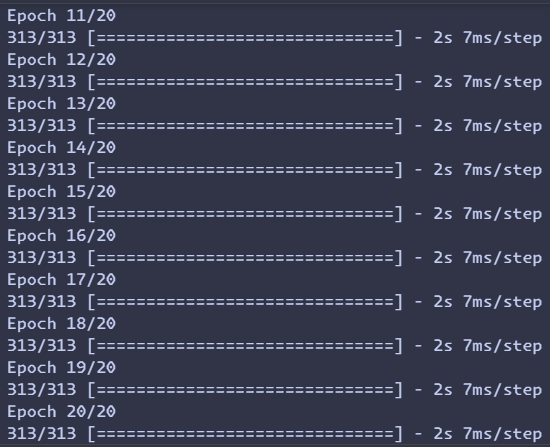
\includegraphics[width=0.5\textwidth]{Proposal/9070XTModelTraining.png}
    \caption{Training time for a CNN on the CIFAR10 dataset using an RX 9070 XT (7ms/step, 2s/epoch).\label{fig:GPUComparisonB}}
\end{figure}

\endgroup 